%& -shell-escape
%
% `template_basic.tex' - A bare-bones example of using the AIAA class.
%                        For a more advanced usage, see `template_advanced.tex'.
%
% Typical processing for PostScript (PS) output:
%
%  latex template_basic
%  latex template_basic   (repeat as needed to resolve references)
%
%  xdvi template_basic    (onscreen draft display)
%  dvips template_basic   (postscript)
%  gv template_basic.ps   (onscreen display)
%  lpr template_basic.ps  (hardcopy)
%
% With the above, only Encapsulated PostScript (EPS) images can be used.
%
% Typical processing for Portable Document Format (PDF) output:
%
%  pdflatex template_basic
%  pdflatex template_basic      (repeat as needed to resolve references)
%
%  acroread template_basic.pdf  (onscreen display)
%
% If you have EPS figures, you will need to use the epstopdf script
% to convert them to PDF because PDF is a limmited subset of EPS.
% pdflatex accepts a variety of other image formats such as JPG, TIF,
% PNG, and so forth -- check the documentation for your version.
%
% If you do *not* specify suffixes when using the graphicx package's
% \includegraphics command, latex and pdflatex will automatically select
% the appropriate figure format from those available.  This allows you
% to produce PS and PDF output from the same LaTeX source file.
%
% To generate a large format (e.g., 11"x17") PostScript copy for editing
% purposes, use
%
%  dvips -x 1467 -O -0.65in,0.85in -t tabloid template_basic
%a
% For further details and support, read the Users Manual, aiaa.pdf.
%
% This software is released under the terms of the LaTeX Project Public
% License.  Copyright (C) 2004 by Bil Kleb, Bill Wood, and Erich Knausenberger.
\documentclass[times,12pt]{article}% insert '[draft]' option to show overfull boxes
\usepackage{python}
%\documentclass[]{aiaa-tc}% insert '[draft]' option to show overfull boxes
\usepackage[english]{babel} % English language/hyphenation
\usepackage{amsmath,amsfonts,amsthm} % Math packages
\usepackage{graphicx}
\usepackage{comment}
\usepackage[dvipsnames]{xcolor}
\usepackage{pdfpages}
\usepackage[utf8]{inputenc}
 
\usepackage{listings}
\usepackage{color}
 
\definecolor{codegreen}{rgb}{0,0.6,0}
\definecolor{codegray}{rgb}{0.5,0.5,0.5}
\definecolor{codepurple}{rgb}{0.58,0,0.82}
\definecolor{backcolour}{rgb}{0.95,0.95,0.92}
\usepackage{color}

\lstdefinestyle{mystyle}{
    backgroundcolor=\color{backcolour},   
    commentstyle=\color{codegreen},
    keywordstyle=\color{magenta},
    numberstyle=\tiny\color{codegray},
    stringstyle=\color{codepurple},
    basicstyle=\footnotesize,
    breakatwhitespace=false,         
    breaklines=true,                 
    captionpos=b,                    
    keepspaces=true,                 
    numbers=left,                    
    numbersep=5pt,                  
    showspaces=false,                
    showstringspaces=false,
    showtabs=false,                  
    tabsize=2
}
 
\lstset{style=mystyle}

\usepackage{wasysym}
\usepackage{subcaption}
\usepackage{vhistory}
\usepackage[colorlinks=true, pdfstartview=FitV, linkcolor=blue,citecolor=red, urlcolor=red]{hyperref}
\usepackage{float}
\usepackage[font={footnotesize}]{caption}
\usepackage[autoplay]{animate}
\usepackage{movie15}
% in documenet
\newcommand{\MC}{\mathcal}
\usepackage[margin=1.in]{geometry}
 \title{Research Notes}
 \setlength{\abovecaptionskip}{1pt plus 0pt minus 50pt}
\newcommand{\BG}{\boldsymbol}
\newcommand{\CONVRU} {\sum_{\substack{ \mathbf{p} + \mathbf{q} = \mathbf{k} \\ \mathbf{p} \in F, \mathbf{q} \in  G }} }
\usepackage[toc,page]{appendix}


 % Data used by 'handcarry' option if invoked
 %\AIAApapernumber{YEAR-NUMBER}
 %\AIAAconference{Conference Name, Date, and Location}
 %\AIAAcopyright{\AIAAcopyrightD{YEAR}}

 % Define commands to assure consistent treatment throughout document
 \newcommand{\eqnref}[1]{(\ref{#1})}
 \newcommand{\class}[1]{\texttt{#1}}
 \newcommand{\package}[1]{\texttt{#1}}
 \newcommand{\file}[1]{\texttt{#1}}
 \newcommand{\BibTeX}{\textsc{Bib}\TeX}

\newcommand{\pd}[2]{\frac{\partial #1}{\partial #2}}
\newcommand{\be}{\ensuremath{{\boldsymbol\beta}}\xspace}
\newcommand{\ret}{\ensuremath{ Re_{\theta} \xspace}}
\newcommand{\bm}{\ensuremath{{\boldsymbol\beta_{MAP}}}\xspace}
\newcommand{\ufine}{\ensuremath{\hat{\color{red} \mathbf{u} }}}
\newcommand{\ufull}{\ensuremath{\mathbf{u}}}
\newcommand{\ucoarse}{\ensuremath{\tilde{\color{blue} \mathbf{u} }}}
\newcommand{\afine}{\ensuremath{{\hat{\color{red} \mathbf{a} }_r}}}
\newcommand{\acoarse}{\ensuremath{{\tilde{\color{blue} \mathbf{a} }}}}
\newcommand{\afull}{\ensuremath{{\color{black} \mathbf{a} }}}
\newcommand{\wfine}{\ensuremath{\hat{\color{red} w } } }
\newcommand{\wcoarse}{\ensuremath{\tilde{\color{blue} w } } }
\newcommand{\wvcoarse}{\ensuremath{\tilde{\color{blue} w } } }
\newcommand{\kcoarse}{\ensuremath{\tilde{\color{blue} k } } }
\newcommand{\omegacoarse}{\ensuremath{\tilde{\color{blue} \omega } } }
\newcommand{\Vfine}{\ensuremath{{\color{red} \mathbf{\hat{V}}}}}
\newcommand{\Vcoarse}{\ensuremath{{\color{blue} \mathbf{\tilde{V}}}}}
\newcommand{\Vfull}{\ensuremath{ \mathbf{V}}}
\newcommand{\Picoarse}{\ensuremath{{\color{blue} \mathbf{\tilde{\Pi}}}}}
\newcommand{\Pifine}{\ensuremath{{\color{red} \mathbf{\hat{\Pi}}}}}
\begin{document}




%----------------------------------------------------------------------------------------
%	PROBLEM 1
%----------------------------------------------------------------------------------------
\section{PyDG Manual}
PyDG is a high-order discontinuous Galerkin code written in python. The purpose of this document will be to familiarize the reader with PyDG. We will first discuss how to run the code, and then provide details into the inner workings of the code.

\subsection{Running PyDG}
To run PyDG, we need to construct an input file. This input file specifies things like the grid, order of accuracy, equation sets, etc.  A sample inputfile for the isentropic vortex is given:
%and requires specification of:
%\begin{itemize}
%\item The $N_{el}$ array. This must be a 1D vector of length 4. Entries are elements in $x,y,z,t$
%\item The $order$ array. Arguments are order of accuracy in each direciton
%\item The $quadpoints$ array. Arguments are the number of quad points in each direction
%\item The viscosity, $\mu$. This must be specified even if inviscid.
%\item The grid, x,y, and $z$. These must be passed in the format of a 3D array.
%\end{itemize}
\begin{lstlisting}
import numpy as np
import sys
sys.path.append("../../src_spacetime") #link the source directory for PyDG
from ic_functions_premade import vortexICS  #import the IC function
def savehook(main): # function called every save_freq iterations
  pass
## Make square grid
L = 10.                       #|  length
Nel = np.array([32,32,1,1])   #|  elements in x,y,z,t
order =np.array([2,2,1,1])    #|  spatial order
quadpoints = order*1.         #|  number of quadrature points
mu = 0.                       #|  viscocity
x = np.linspace(0,L,Nel[0]+1) #|  x, y, and z
y = np.linspace(0,L,Nel[1]+1) #|
z = np.linspace(0,L,Nel[2]+1) #|
x,y,z = np.meshgrid(x,y,z,indexing='ij')
t = 0                         #|  simulation start time
dt = 0.0125                   #|  time step
et = 10.                      #|  simulation end time
save_freq = 10.              #|  frequency to save output and print to screen
eqn_str = 'Navier-Stokes'   #|  equation set
schemes = ('roe','Inviscid')   #|  inviscid and viscous flux schemes
procx = 2                         #|  processor decomposition in x
procy = 2      #|  same in y. Note procx*procy needs to equal total number of procs

## Boundary conditions
right_bc = 'periodic' 
left_bc = 'periodic'
top_bc = 'periodic'
bottom_bc = 'periodic'
front_bc = 'periodic'
back_bc = 'periodic'

## Arguments for boundary conditions
right_bc_args = []
left_bc_args = []
top_bc_args = []
bottom_bc_args = []
front_bc_args = []
back_bc_args = []

# creation of BCs array for the solver
BCs = [right_bc,right_bc_args,top_bc,top_bc_args,left_bc,left_bc_args,bottom_bc,bottom_bc_args,front_bc,front_bc_args,back_bc,back_bc_args]

# Misc strings that currently are required (from combustion)
source_mag= False
mol_str = False				   #|

# Time stepping. The linear and nonlinear solvers are only used if implicit
time_integration = 'SSP_RK3'
linear_solver_str = 'GMRes'
nonlinear_solver_str = 'Newton'

#== Assign initial condition function. Note that you can alternatively define this here
#== layout is my_ic_function(x,y,z), where x,y,z are the quad points
IC_function = vortexICS                #|
                                   #|
execfile('../../src_spacetime/PyDG.py')      #|  call the solver
\end{lstlisting}
\noindent To PyDG with the above script, move to the directory of "inputfile.py" and type into the command line:
\begin{lstlisting}[language=bash]
  $ mpirun -np 4 python inputfile.py
\end{lstlisting}
\subsubsection{Post Processing}
Running PyDG will lead to the creation of a folder called "Solution" in the directory where the inputfile is. In this "Solution" directory, PyDG will put saved states of the solution - for example "npsol0.npz". These states are saved every "$save_freq$" iterations; this is defined in the input deck. The solution files are saved in ".npz" format and may be visualized in python. A post processing script that converts the solution files to ".vts" files for visualization in paraview is also available. To run this script, one should move to the "Solution" directory and run the postProcessing.py script with the appropriate equation set that is present in the src\_spacetime folder:
\begin{lstlisting}[language=bash]
  $ cd Solution 
  $ python (PyDG home directory)/src_spacetime/postProcessing.py (Eqn set)
\end{lstlisting}
Currently implemented equation sets are:
\begin{enumerate}
\item Navier-Stokes
\begin{itemize}
\item This runs the script for the classic Navier-Stokes (or Euler) equations. It outputs fields of $\rho, \rho u_i, $ and $\rho E$.
\end{itemize}
\item Entropy
\begin{itemize}
\item This runs the script for the Navier-Stokes equations with entropy variables. It outputs fields of $\rho, \rho u_i, $ and $\rho E$.
\end{itemize}
\item Scalar
\begin{itemize}
\item This runs the script for a scalar equation. It outputs the field with the name $u$.
\end{itemize}
\end{enumerate}

\subsection{The Code}
Here we dive into details about how the code works.

\subsubsection{Spatial Discretization: The Discontinuous Galerkin Approach}
PyDG utilizes Legendre polynomials for its spatial discretization. The Legendre polynomials consist of a hierarchical set of polynomials and are orthogonal on the unit cube. For multidimensional problems, PyDG uses tensor products. The remainder of this section will outline the discontinuous Galerkin approach;

We consider the system of conservation laws,
\begin{equation}\label{eq:genEq}
\frac{\partial \mathbf{u}}{\partial t} +  \nabla \cdot \mathbf{F} = 0
\end{equation}
with $\mathbf{x} \in \Omega$. In the discontinuous Galerkin approach, the domain $\Omega$ is subdivided into individual elements, $\Omega_k$. The state variable $\mathbf{u}$ is then approximated by basis functions over $\Omega$,
$$\mathbf{u}(\mathbf{x},t) = \sum_{k=0}^{N-1} \sum_{j = 0}^p \mathbf{a}_{j,k}(t) \mathbf{w}_{k,j}(\mathbf{x}),$$
where $\mathbf{a}$ are the basis coefficients and $\mathbf{w}$ are the basis functions. Note that in the DG approach, the basis functions have local support and are hence discontinuous between the elements. 

The DG approach proceeds by multiplying Eq.~\ref{eq:genEq} by the basis functions and integrating over the support of each basis function,
\begin{equation}\label{eq:genEq2}
\int_{\Omega_k} \mathbf{w}_{k,j} \bigg[\frac{\partial \mathbf{u}}{\partial t}  +  \nabla \cdot \mathbf{F} \bigg] d\Omega = 0.
\end{equation}
The flux term is then integrated by parts. This integration by parts couples all the elements and establishes the finite-volume aspect of the DG approach. One has~\cite{kfid_cfdnotes},
\begin{equation}\label{eq:genEq3}
\int_{\Omega_k} \mathbf{w}_{k,j}\frac{\partial \mathbf{u}}{\partial t} d\Omega   - \int_{\Omega_k} \nabla \mathbf{w}_{k,j} \cdot \mathbf{F}  d\Omega  + \int_{d \Omega_k} \mathbf{w}_{k,j}^+ \hat{\mathbf{F}} (\mathbf{u}^+,\mathbf{u}^-, \hat{n}) dl  = 0,
\end{equation}
where $+$ and $-$ refers to the element interior and exterior, respectively. The term $ \hat{\mathbf{F}} $ is the numerical flux between the faces. 

The numerical implementation of the DG method has three parts:
\begin{enumerate}
\item Evaluation of the volumetric integrals (second term in Eq.~\ref{eq:genEq3}.)
\item Evaluation of the fluxes (third term in Eq.~\ref{eq:genEq3}.)
\item Coupling to a time marching scheme.
\end{enumerate}




\subsection{Code Layout}
The general structure of the code is shown in Figure~\ref{fig:layout}. The code is driven by an inputfile, callled "inputfile.py". In this file, aspects such as the grid, order of accuracy, equation set, boundary conditions, etc. are defined. This file proceeds to call the driving script, "PyDG.py". The script "PyDG.py" first initializes variables and equation sets and then runs the main time loop. Inside the time loop, the script "timeSchemes.py" is called. The "timeSchemes.py" script contains the time scheme routines. In each stage of a time scheme routine, the script "turb\_model.py" is called. This "turb\_models.py" script contains manipulations that are performed in turbulence models. Note that the code mainly focuses on residual-based-type closure models and as such the "turb\_models.py" script exists outside of the traditional RHS evaluation files. The "turb\_models.py" script will call the script "DG\_functions.py". This script is responsible for calculating the flux and volume terms in a DG formulation. 
\begin{figure}[h]
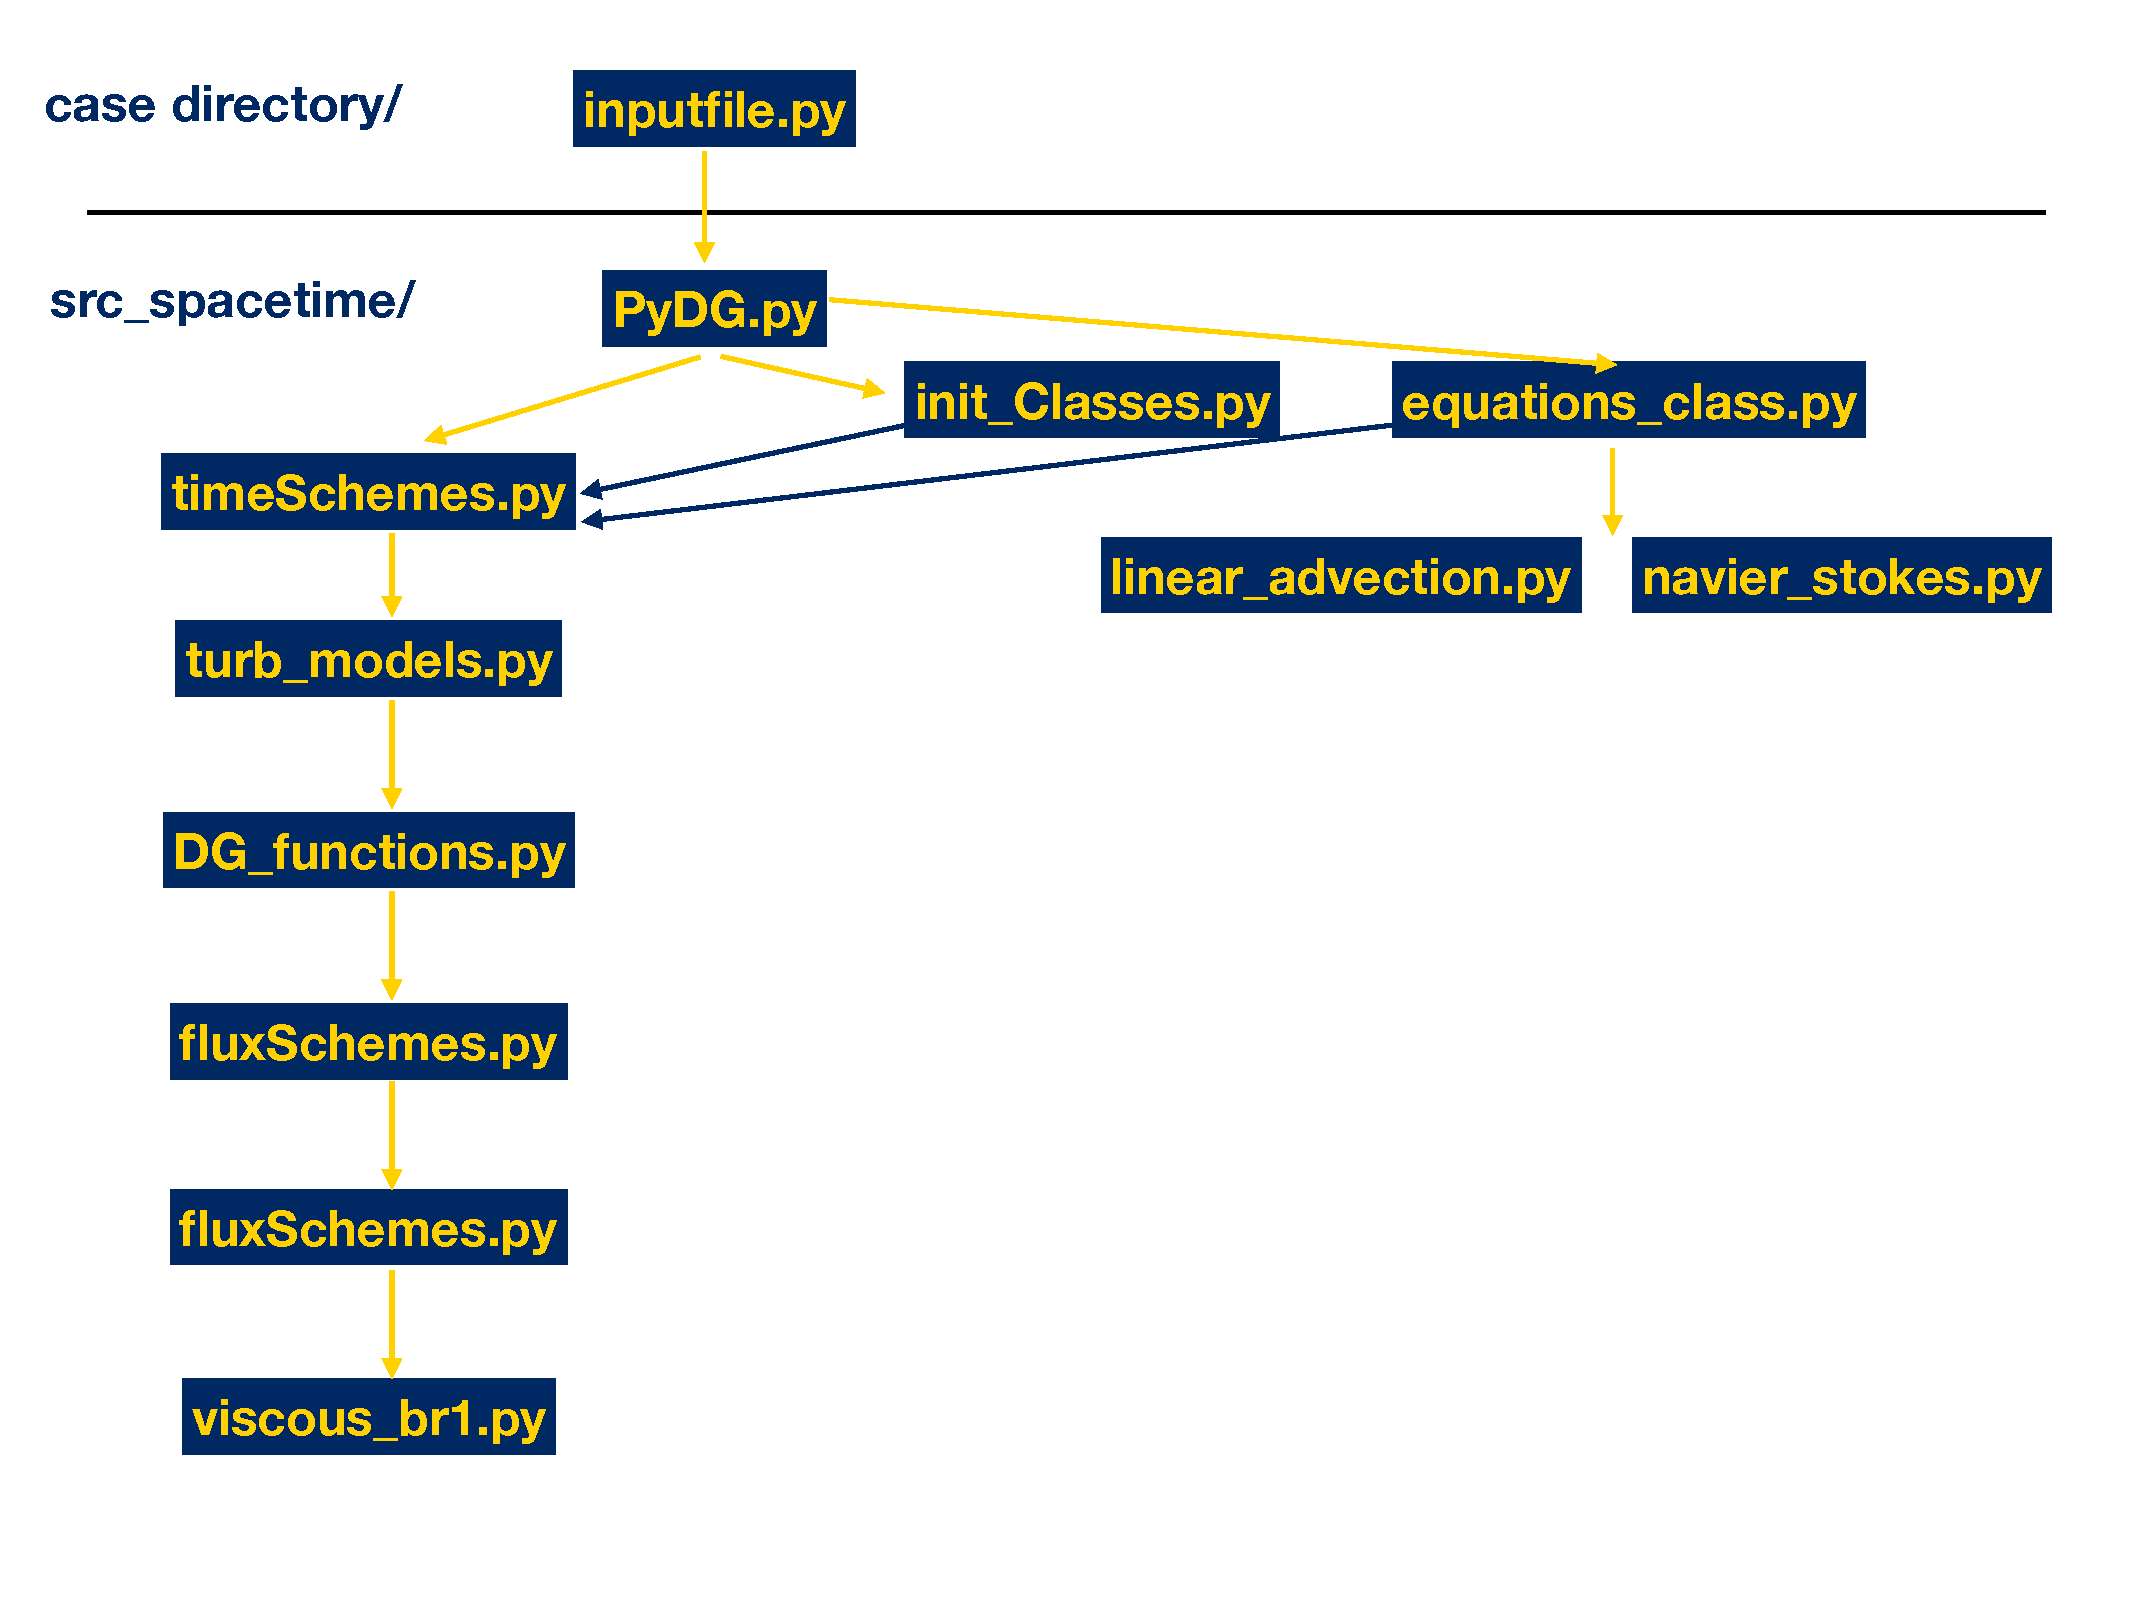
\includegraphics[trim={0.05cm 0 1.75cm 1cm},clip,width=1.\linewidth]{figs/pydg_layout.pdf}
\caption{Layout for PyDG. Yellow arrows are function calls, blue arrows are passed classes}
\label{fig:layout}
\end{figure}
 
 
\subsection{General Dimension of Variables}
The variables in PyDG primarily consist of variables in modal space and variables in physical space. The variables in modal space, which are typically referenced by a command similar to "classname.a", are of dimension,
$$classname.a = N_{vars} \times N_{px} \times N_{py}  \times N_{pz}  \times N_{pt} \times N_{elx} \times N_{ely}  \times N_{elz}  \times N_{elt}.$$
Yes, they are $8D$ arrays! The variable $N_{vars}$ is the number of unknown variables (eg. $5$ for compressible Euler). The term $N_{px}$ is the order of the polynomial in the $x$ direction, with $N_{py}$, $N_{pz}$, and $N_{pt}$ being the same for the $y$, $z$, and temporal direction, respectively. Similarly, the $N_{el}$ terms refer to the number of elements in each direction. 

Variables in physical space have a similar structure. Typically referenced by a command similar to "classname.u", they are of dimension
$$classname.u = N_{vars} \times N_{qx} \times N_{qy}  \times N_{qz}  \times N_{qt} \times N_{elx} \times N_{ely}  \times N_{elz}  \times N_{elt}.$$
Similar to $N_{px}$, terms such as $N_{qx}$ refer to the number of quadrature points in each direction. Typically for the Euler equations, one uses twice the quadrature points as the order of the polynomial.

\subsection{The variables class}
The variables class, typically assigned "main", is the primary class used in the solver. The variables class is defined in "init\_Classes.py". Variables contains several important subvariables and subclasses
\begin{itemize}
\item variables.a: This is a subclass that represents the main state variables. 
\begin{itemize}
\item a.a: These are the Legendre coefficients associated with the state variable in $a$. The dimensions are 
$$a.a = N_{vars} \times N_{px} \times N_{py}  \times N_{pz}  \times N_{pt} \times N_{elx} \times N_{ely}  \times N_{elz}  \times N_{elt} $$
\item a.u: These are the physical space values associated with the state variable in $a$. The dimensions are 
$$a.u = N_{vars} \times N_{qx} \times N_{qy}  \times N_{qz}  \times N_{qt} \times N_{elx} \times N_{ely}  \times N_{elz}  \times N_{elt} $$
\end{itemize}

\end{itemize}

\end{document}







